\documentclass[10pt,a4paper]{article}
\usepackage[latin1]{inputenc}
\usepackage{amsmath}
\usepackage{xcolor}
\usepackage{amsfonts}
\usepackage{amssymb}
\usepackage{graphicx}
\usepackage{listings}
\usepackage[margin=1in]{geometry}
\DeclareGraphicsExtensions{.pdf,.png,.jpg}



\lstset{
	frame=single,
	breaklines=true,
	postbreak=\raisebox{0ex}[0ex][0ex]{\ensuremath{\color{red}\hookrightarrow\space}}
	}
	\lstdefinelanguage{numpy}{
		keywords = {
			and,del,from,not,while,
			as,elif,global,or,with,
			assert,else,if,pass,yield,
			break,except,import,print,
			class,exec,in, raise,continue,
			finally,is, return,def,for,
			lambda,try
			},
			morekeywords = {numpy,fft,mean}
			}

\author{Mohammad A.Raji, Alok Hota}
\title{3D N-Body Simulation with CUDA and ThreeJS}

\begin{document}
	\maketitle
	
	\section{Introduction}
	N-body simulation, is a simulation of the effects of physical forces between particles in a dynamical system, and is used in many areas such as: astronomy, physics, chemistry, etc. The simulation is very time consuming due to the large number of particles and the need to calculate the force between all combinations. 
	
	In this work, we implement a serial and a parallel version of the simulation to show the effectiveness of GPU parallelization for the problem and also provide an interactive web interface for viewing the simulation results. Our simulation is tested with a maximum number of 1024 particles for 10000 timesteps. 
	\section{Method}
	
	\section{User Interface}
	To view the simulation results, we created a web interface that receives the simulation results as a \textbf{csv} file and renders it as a simulation in a 3D environment using ThreeJS - the WebGL based library.
	
	The presented web interface provides the following the features: 
	\begin{itemize}
		\item Panning and zooming in a 3D environment
		\item Pausing and playing the simulation 
		\item Slow motion option
		\item Manual and automatic rotation option
	\end{itemize}
	
	A screenshot of our web interface is shown in Figure \ref{scr}.
	\begin{figure}
		\centering
		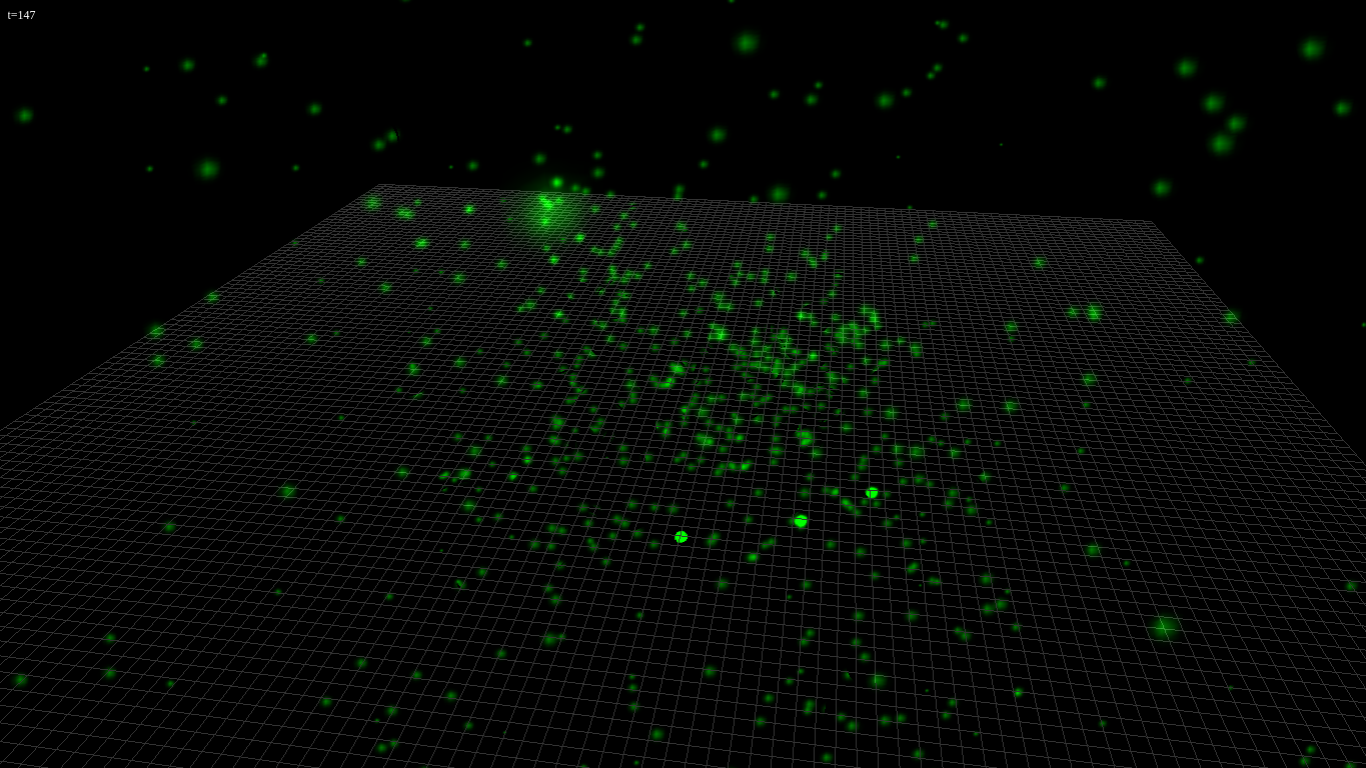
\includegraphics[scale=0.3]{scr.png}
		\caption{Web interface for our 3D n-body simulation}
		\label{scr}
	\end{figure}
	
	\section{Evaluation}
	We tested our implementations on a machine with four Xeon CPUs and an Nvidia Quadro FX3800 GPU with 192 cores. 
	
	For evaluation, the runtime of the serial and parallel implementations are compared. The values used for the number of particles in this comparison were 64, 128, 256, 512 and 1024. The implementations created a simulation file for 10000 timesteps. The large number of timesteps simulated, provides a flexible way to increase or decrease the speed of the visualization if needed. The results are shown in \textbf{Figure [?]}.
	
	\pagebreak
	
	\section{Appendix A: Installation}
		The code for our work is available at http://github.com/ahota/nobody and can be downloaded using Git by running: \texttt{git clone http://github.com/ahota/nobody}.
		
		\subsection{Dependencies}
		For running the simulation, the only dependency is a machine with an Nvidia GPU that supports CUDA. For running the web interface, Python's Flask micro-framework needs to be installed to be able to serve the simulation interface as a web server. You can install Flask by running \texttt{sudo pip install flask}. 
		
		\subsection{Compiling}
		The serial and the parallel implementations can be compiled by running \texttt{./src/simulator/compile.sh}. 
		
		\subsection{Running the simulation}
		For the serial version, run \texttt{./src/simulator/nbody\_cpu}.
		The parallel version can be executed by running \texttt{./src/simulator/nbody\_cuda}.
		
		The parallel version provides an \texttt{nbd} file that can be fed into a script as input to make it ready for visualization. This can be done by running \texttt{python scale\_for\_vis.py <filename>}, where filename is the name of the file made by running the simulation. This script creates a simulation.csv file that has to be copied to \texttt{./ui/data/} for the web server to pick up. The python web server starts and serves at \texttt{localhost:5000} by running \texttt{python run.py} in \texttt{./src/ui/}. From now on, any web browser can view the simulation on http://localhost:5000.
		
	\section{Appendix B: Header file}
	\begin{lstlisting}[language=c]
	#include<stdio.h>
	#include<stdlib.h>
	#include<string.h>
	#include<unistd.h>
	#include<math.h>
	#include<sys/time.h>
	#include<time.h>
	
	#define CMAX       1496         //+-1 AU * 10e-5
	#define CMIN      -1496
	#define MMAX       9e2         //approximately mass of Ceres
	#define MMIN       14e1         //approximately mass of Bennu
	#define AMAX       1000
	#define AMIN      -1000
	#define VC         299792458    //speed of light
	
	#define EPSILON2   0.5f         //softener used to prevent r^2 -> 0
	
	#define DEF_BODIES 256
	#define G          1.0f//6.673e-11f   //gravitational constant
	#define DEF_DELTA  0.1f
	#define DEF_STEPS  10000
	
	//Lazy programming
	int NUM_BODIES, NUM_STEPS;
	float DELTA_T;
	
	//tools
	int parse_args(int argc, char **argv);
	int output = 1;
	
	//parameter functions
	float rand_acceleration();
	float rand_coordinate();
	float rand_mass();
	
	//timing functions and struct
	typedef struct {
		struct timeval start;
		struct timeval end;
	} timer;
	void start_timer(timer *t);
	void stop_timer(timer *t);
	float elapsed_time(timer *t);
	\end{lstlisting}
	
	\section{Appendix B: Serial version}
	\begin{lstlisting}[language=c]
	#include "nbody.h"
	
	//CPU-specific structs and functions
	typedef struct {
		float x;
		float y;
		float z;
	} float3;
	
	typedef struct {
		float x;
		float y;
		float z;
		float w;
	} float4;
	void interact(float4 *body_i, float4 *body_j, float3 *acc_i, float4 *inter_i);
	
	int main(int argc, char **argv) {
		//Get parameters, if any, from user
		NUM_BODIES = DEF_BODIES;
		NUM_STEPS  = DEF_STEPS;
		DELTA_T    = DEF_DELTA;
		int status = parse_args(argc, argv);
		if(status)
		return status;
		
		int i, j, t;
		srand(time(NULL));
		timer perf_timer;
		timer total_timer;
		
		printf("Creating bodies...\n");
		
		float4 *pos_mass;
		float4 *intermediate;
		float3 *acc;
		
		printf("Allocating memory...\n");
		
		start_timer(&total_timer);
		pos_mass     = (float4 *)malloc(NUM_BODIES * sizeof(float4));
		intermediate = (float4 *)malloc(NUM_BODIES * sizeof(float4));
		acc          = (float3 *)malloc(NUM_BODIES * sizeof(float3));
		
		printf("Initializing bodies...\n");
		
		for(i = 0; i < NUM_BODIES; i++) {
			pos_mass[i].x = rand_coordinate();
			pos_mass[i].y = rand_coordinate();
			pos_mass[i].z = rand_coordinate();
			pos_mass[i].w = rand_mass();
		}
		
		printf("SIMULATION SETTINGS:\n");
		printf("  bodies  = %d\n", NUM_BODIES);
		printf("  steps   = %d\n", NUM_STEPS);
		printf("  delta t = %f\n", DELTA_T);
		
		printf("Running simulation...\n");
		
		start_timer(&perf_timer);
		for(t = 0; t < NUM_STEPS; t++) {
			for(i = 0; i < NUM_BODIES; i++) {
				for(j = 0; j < NUM_BODIES, j != i; j++) {
					interact(&pos_mass[i], &pos_mass[j], &acc[i], &intermediate[i]);
				}
			}
			//Update positions
			for(i = 0; i < NUM_BODIES; i++) {
				pos_mass[i] = intermediate[i];
			}
		}
		stop_timer(&perf_timer);
		stop_timer(&total_timer);
		
		printf("Simulation runtime:\t%f s\n", elapsed_time(&perf_timer));
		printf("Total runtime:\t%f s\n", elapsed_time(&total_timer));
		
		if(output) {
			time_t raw_time;
			struct tm *current_time;
			time(&raw_time);
			current_time = localtime(&raw_time);
			char *filename = (char *)malloc(64);
			sprintf(filename, "cpu_%02d%02d%02d_%02d%02d%02d.nbd", 
			current_time->tm_year%100, current_time->tm_mon,
			current_time->tm_mday, current_time->tm_hour,
			current_time->tm_min, current_time->tm_sec);
			
			printf("Saving to %s...\n", filename);
			
			FILE *outfile = fopen(filename, "w");
			if(outfile == NULL)
			fprintf(stderr, "Error opening file\n");
			else {
				fprintf(outfile, "Final output:\n");
				
				fprintf(outfile, "i\tx\t\ty\t\tz\n");
				fprintf(outfile, "---\n");
				for(i = 0; i < NUM_BODIES; i++) {
					fprintf(outfile, "%d\t%f\t%f\t%f\n", i, pos_mass[i].x,
					pos_mass[i].y, pos_mass[i].z);
				}
				fclose(outfile);
			}
		}
		
		printf("Done.\n");
		
		return 0;
	}
	
	void interact(float4 *body_i, float4 *body_j, float3 *acc_i, float4 *inter_i) {
		//calculate distance components
		float3 d;
		d.x = body_j->x - body_i->x;
		d.y = body_j->y - body_i->y;
		d.z = body_j->z - body_i->z;
		
		//use episilon softener
		//  r^2 + epsilon^2
		float denominator = d.x * d.x + d.y * d.y + d.z * d.z + EPSILON2;
		//cube and sqrt to get (r^2 + epsilon^2)^(3/2)
		denominator = sqrt( denominator * denominator * denominator );
		
		float acc = G * body_j->w / denominator;
		
		//update acceleration
		acc_i->x += acc * d.x * DELTA_T;
		acc_i->y += acc * d.y * DELTA_T;
		acc_i->z += acc * d.z * DELTA_T;
		
		//update position of body i
		inter_i->x = body_i->x + acc_i->x;
		inter_i->y = body_i->y + acc_i->y;
		inter_i->z = body_i->z + acc_i->z;
		inter_i->w = body_i->w;
	}
	
	int parse_args(int argc, char **argv) {
		int i;
		for(i = 1; i + 1 <= argc; i += 2) {
			if(strcmp(argv[i], "-h") == 0) {
				printf("Usage: %s [-b num_bodies] [-s num_steps] [-t delta_t] \ [-o]\n", argv[0]);
				return 1;
			}
			else if(strcmp(argv[i], "-b") == 0) {
				NUM_BODIES = atoi(argv[i + 1]);
			}
			else if(strcmp(argv[i], "-s") == 0) {
				NUM_STEPS  = atoi(argv[i + 1]);
			}
			else if(strcmp(argv[i], "-t") == 0) {
				DELTA_T    = atof(argv[i + 1]);
			}
			else if(strcmp(argv[i], "-o") == 0) {
				output     = 0;
			}
			else {
				fprintf(stderr, "Error: unsupported flag %s\n", argv[i]);
				return -1;
			}
		}
		return 0;
	}
	
	float rand_coordinate() {
		return ((float)rand() / (float)RAND_MAX) * (CMAX - CMIN) + CMIN;
	}
	
	float rand_acceleration() {
		return ((float)rand() / (float)RAND_MAX) * (AMAX - AMIN) + AMIN;
	}
	
	float rand_mass() { 
		return ((float)rand() / (float)RAND_MAX) * (MMAX - MMIN) + MMIN;
	}
	
	void start_timer(timer *t) {
		gettimeofday( &(t->start), NULL);
	}
	
	void stop_timer(timer *t) {
		gettimeofday( &(t->end), NULL);
	}
	
	float elapsed_time(timer *t) {
		return (float) (t->end.tv_sec  - t->start.tv_sec)  + 
		(t->end.tv_usec - t->start.tv_usec) /
		1000000.0;
	}
	\end{lstlisting}
	
	\section{Appendix C: Parallel version}
	
	\begin{lstlisting}[language=c]
	#include "nbody.h"
	#include<cuda.h>
	
	//CUDA-specific vars and functions
	__device__ int NBODIES;
	__device__ float DT;
	__global__ void main_nbody_kernel(float4 *dev_pos_mass, float3 *dev_acc,
	float3 *dev_output, int cur_step);
	__device__ void tile_nbody_kernel(float4 *my_pos_mass, float3 *my_acc);
	__device__ void force_kernel(float4 *body_i, float4 *body_j,
	float3 *acc_i);
	
	int main(int argc, char **argv) {
		//Get parameters, if any, from user
		NUM_BODIES = DEF_BODIES;
		NUM_STEPS  = DEF_STEPS;
		DELTA_T    = DEF_DELTA;
		int status = parse_args(argc, argv);
		if(status)
		return status;
		cudaMemcpyToSymbol(NBODIES, &NUM_BODIES, sizeof(int), 0, 
		cudaMemcpyHostToDevice);
		cudaMemcpyToSymbol(DT, &DELTA_T, sizeof(int), 0, 
		cudaMemcpyHostToDevice);
		
		int i;
		srand(time(NULL));
		timer perf_timer;
		timer total_timer;
		
		printf("Creating bodies...\n");
		
		float4 *host_pos_mass, *dev_pos_mass;
		float3 *host_acc, *dev_acc;
		float3 *host_output, *dev_output;
		
		printf("Allocating host memory...\n");
		
		start_timer(&total_timer);
		host_pos_mass = (float4 *)malloc(NUM_BODIES * sizeof(float4));
		host_acc      = (float3 *)malloc(NUM_BODIES * sizeof(float3));
		host_output   = (float3 *)malloc(NUM_BODIES * NUM_STEPS * sizeof(float3));
		
		printf("Allocating device memory...\n");
		
		cudaMalloc((void **)&dev_pos_mass, NUM_BODIES * sizeof(float4));
		cudaMalloc((void **)&dev_acc, NUM_BODIES * sizeof(float3));
		cudaMalloc((void **)&dev_output, NUM_BODIES * NUM_STEPS * sizeof(float3));
		
		printf("Initializing bodies...\n");
		
		for(i = 0; i < NUM_BODIES; i++) {
			host_pos_mass[i].x = rand_coordinate();
			host_pos_mass[i].y = rand_coordinate();
			host_pos_mass[i].z = rand_coordinate();
			host_pos_mass[i].w = rand_mass();
		}
		
		printf("SIMULATION SETTINGS:\n");
		printf("  bodies  = %d\n", NUM_BODIES);
		printf("  steps   = %d\n", NUM_STEPS);
		printf("  delta t = %f\n", DELTA_T);
		
		/*
		printf("Initial positions and masses:\n");
		for(i = 0; i < NUM_BODIES; i++) {
			printf("%d:\t%f\t%f\t%f\n", i, host_pos_mass[i].x, host_pos_mass[i].y,
			host_pos_mass[i].z, host_pos_mass[i].w);
		}
		*/
		
		printf("Copying to device...\n");
		
		cudaMemcpy(dev_pos_mass, host_pos_mass, NUM_BODIES * sizeof(float3),
		cudaMemcpyHostToDevice);
		cudaMemcpy(dev_acc, host_acc, NUM_BODIES * sizeof(float3),
		cudaMemcpyHostToDevice);
		cudaMemcpy(dev_output, host_output, NUM_BODIES * NUM_STEPS * sizeof(float3),
		cudaMemcpyHostToDevice);
		
		printf("Running kernel...\n");
		
		start_timer(&perf_timer);
		int block_size = (NUM_BODIES < 16) ? 4 : (NUM_BODIES < 256) ? 16 : 32;
		int grid_size  = NUM_BODIES / block_size;
		int mem_size = (block_size+1) * sizeof(float4);
		printf("KERNEL SETTINGS:\n");
		printf("  bodies    = %d\n", NUM_BODIES);
		printf("  tile size = %d\n", block_size);
		printf("  grid size = %d\n", grid_size);
		for(i = 0; i < NUM_STEPS; i++) {
			main_nbody_kernel<<<grid_size, block_size, mem_size>>>(dev_pos_mass,
			dev_acc, dev_output, i);
		}
		stop_timer(&perf_timer);
		
		printf("Simulation runtime:\t%f s\n", elapsed_time(&perf_timer));
		
		printf("Copying to host...\n");
		
		cudaMemcpy(host_output, dev_output, NUM_BODIES * NUM_STEPS * sizeof(float3),
		cudaMemcpyDeviceToHost);
		cudaFree(dev_pos_mass);
		cudaFree(dev_acc);
		cudaFree(dev_output);
		stop_timer(&total_timer);
		
		printf("Total runtime:\t%f s\n", elapsed_time(&total_timer));
		
		if(output) {
			time_t raw_time;
			struct tm *current_time;
			time(&raw_time);
			current_time = localtime(&raw_time);
			char *filename = (char *)malloc(64);
			sprintf(filename, "cuda_%02d%02d%02d_%02d%02d%02d.nbd", 
			current_time->tm_year%100, current_time->tm_mon,
			current_time->tm_mday, current_time->tm_hour,
			current_time->tm_min, current_time->tm_sec);
			
			printf("Saving to %s...\n", filename);
			
			FILE *outfile = fopen(filename, "w");
			if(outfile == NULL)
			fprintf(stderr, "Error opening file\n");
			else {
				//printf("%f\n", host_output[0].x);
				fprintf(outfile, "%d,%d\n", NUM_BODIES, NUM_STEPS);
				for(i = 0; i < NUM_BODIES * NUM_STEPS; i++) {
					fprintf(outfile, "%f,%f,%f\n", host_output[i].x, 
					host_output[i].y, host_output[i].z);
				}
				fclose(outfile);
			}
		}
		
		printf("Done.\n");
		return 0;
	}
	
	__global__ void main_nbody_kernel(float4 *dev_pos_mass, float3 *dev_acc,
	float3 *dev_output, int cur_step) {
		//index into global arrays for this thread's body
		int global_id = blockIdx.x * blockDim.x + threadIdx.x;
		
		//local copies of this body's position, mass, and acceleration
		float4 my_pos_mass = dev_pos_mass[global_id];
		float3 my_acc = dev_acc[global_id];
		
		//copy of position and mass for bodies in the current tile
		extern __shared__ float4 tile_pos_mass[]; 
		
		//iterate over all tiles and update position and acceleration
		//each iteration loads one tile's worth of data from global memory
		//these reads should be coalesced
		int i, tile;
		for(i = 0, tile = 0; i < NBODIES; i += blockDim.x, tile++) {
			//index into global for this thread's body *for this tile*
			int tile_id = tile * blockDim.x + threadIdx.x;
			
			//threads collaborate to load from global for this tile
			tile_pos_mass[threadIdx.x] = dev_pos_mass[tile_id];
			__syncthreads();
			
			//update acceleration for this thread's body for this tile
			tile_nbody_kernel(&my_pos_mass, &my_acc);
			__syncthreads();
		}
		
		//update position for this body
		my_pos_mass.x += my_acc.x;
		my_pos_mass.y += my_acc.y;
		my_pos_mass.z += my_acc.z;
		
		//update global position array
		dev_pos_mass[global_id] = my_pos_mass;
		dev_acc[global_id] = my_acc;
		
		//update global output
		dev_output[cur_step * NBODIES + global_id].x = my_pos_mass.x;
		dev_output[cur_step * NBODIES + global_id].y = my_pos_mass.y;
		dev_output[cur_step * NBODIES + global_id].z = my_pos_mass.z;
	}
	
	__device__ void tile_nbody_kernel(float4 *my_pos_mass, float3 *my_acc) {
		//tile position array from the outer kernel
		//pre-loaded with this tile's positions and masses
		extern __shared__ float4 tile_pos_mass[];
		
		//iterate over each body in the tile and calculate its effect on
		//this thread's body
		int i;
		for(i = 0; i < blockDim.x; i++) {
			force_kernel(my_pos_mass, &tile_pos_mass[i], my_acc);
		}
	}
	
	__device__ void force_kernel(float4 *body_i, float4 *body_j, float3 *acc_i) {
		//calculate distance components
		float3 d;
		d.x = body_j->x - body_i->x;
		d.y = body_j->y - body_i->y;
		d.z = body_j->z - body_i->z;
		
		//use episilon softener
		//  r^2 + epsilon^2
		float denominator = d.x * d.x + d.y * d.y + d.z * d.z + EPSILON2;
		//cube and sqrt to get (r^2 + epsilon^2)^(3/2)
		denominator = sqrt( denominator * denominator * denominator );
		
		float acc = G * body_j->w / denominator;
		
		//update acceleration
		acc_i->x += acc * d.x * DT;
		acc_i->y += acc * d.y * DT;
		acc_i->z += acc * d.z * DT;
	}
	
	int parse_args(int argc, char **argv) {
		int i;
		for(i = 1; i + 1 <= argc; i += 2) {
			if(strcmp(argv[i], "-h") == 0) {
				printf("Usage: %s [-b num_bodies] [-s num_steps] [-t delta_t] \
				[-o]\n", argv[0]);
				return 1;
			}
			else if(strcmp(argv[i], "-b") == 0) {
				NUM_BODIES = atoi(argv[i + 1]);
			}
			else if(strcmp(argv[i], "-s") == 0) {
				NUM_STEPS  = atoi(argv[i + 1]);
			}
			else if(strcmp(argv[i], "-t") == 0) {
				DELTA_T    = atof(argv[i + 1]);
			}
			else if(strcmp(argv[i], "-o") == 0) {
				output     = 0;
			}
			else {
				fprintf(stderr, "Error: unsupported flag %s\n", argv[i]);
				return -1;
			}
		}
		return 0;
	}
	
	float rand_coordinate() {
		return ((float)rand() / (float)RAND_MAX) * (CMAX - CMIN) + CMIN;
	}
	
	float rand_acceleration() {
		return ((float)rand() / (float)RAND_MAX) * (AMAX - AMIN) + AMIN;
	}
	
	float rand_mass() { 
		return ((float)rand() / (float)RAND_MAX) * (MMAX - MMIN) + MMIN;
	}
	
	void start_timer(timer *t) {
		gettimeofday( &(t->start), NULL);
	}
	
	void stop_timer(timer *t) {
		gettimeofday( &(t->end), NULL);
	}
	
	float elapsed_time(timer *t) {
		return (float) (t->end.tv_sec  - t->start.tv_sec)  + 
		(t->end.tv_usec - t->start.tv_usec) /
		1000000.0;
	}
	\end{lstlisting}
	
\end{document}